%%%%%%%%%%%%%%%%%%%%%%%%%%%%%%%%%%%%%%%%%
% Masters/Doctoral Thesis
% LaTeX Template
% Version 2.5 (27/8/17)
%
% This template was downloaded from:
% http://www.LaTeXTemplates.com
%
% Version 2.x major modifications by:
% Vel (vel@latextemplates.com)
%
% This template is based on a template by:
% Steve Gunn (http://users.ecs.soton.ac.uk/srg/softwaretools/document/templates/)
% Sunil Patel (http://www.sunilpatel.co.uk/thesis-template/)
%
% Template license:
% CC BY-NC-SA 3.0 (http://creativecommons.org/licenses/by-nc-sa/3.0/)
%
%%%%%%%%%%%%%%%%%%%%%%%%%%%%%%%%%%%%%%%%%

%----------------------------------------------------------------------------------------
%   PACKAGES AND OTHER DOCUMENT CONFIGURATIONS
%----------------------------------------------------------------------------------------

\documentclass[
12pt, % The default document font size, options: 10pt, 11pt, 12pt
%oneside, % Two side (alternating margins) for binding by default, uncomment to switch to one side
english, % ngerman for German
onehalfspacing, % Single line spacing, alternatives: onehalfspacing or doublespacing
%draft, % Uncomment to enable draft mode (no pictures, no links, overfull hboxes indicated)
%nolistspacing, % If the document is onehalfspacing or doublespacing, uncomment this to set spacing in lists to single
%liststotoc, % Uncomment to add the list of figures/tables/etc to the table of contents
%toctotoc, % Uncomment to add the main table of contents to the table of contents
%parskip, % Uncomment to add space between paragraphs
%nohyperref, % Uncomment to not load the hyperref package
headsepline, % Uncomment to get a line under the header
%chapterinoneline, % Uncomment to place the chapter title next to the number on one line
%consistentlayout, % Uncomment to change the layout of the declaration, abstract and acknowledgements pages to match the default layout
]{MastersDoctoralThesis} % The class file specifying the document structure

\usepackage[utf8]{inputenc} % Required for inputting international characters
\usepackage[T1]{fontenc} % Output font encoding for international characters
\usepackage{amsmath, amssymb}
%\usepackage{mathpazo} % Use the Palatino font by default

\usepackage[backend=bibtex,style=authoryear,natbib=true]{biblatex} % Use the bibtex backend with the authoryear citation style (which resembles APA)

\addbibresource{example.bib} % The filename of the bibliography

\usepackage[autostyle=true]{csquotes} % Required to generate language-dependent quotes in the bibliography

%----------------------------------------------------------------------------------------
%   MARGIN SETTINGS
%----------------------------------------------------------------------------------------

\geometry{
    paper=a4paper, % Change to letterpaper for US letter
    inner=2.5cm, % Inner margin
    outer=3.8cm, % Outer margin
    bindingoffset=.5cm, % Binding offset
    top=1.5cm, % Top margin
    bottom=1.5cm, % Bottom margin
    %showframe, % Uncomment to show how the type block is set on the page
}

%----------------------------------------------------------------------------------------
%   THESIS INFORMATION
%----------------------------------------------------------------------------------------

\thesistitle{Feature Selection for Diffusion-based Inpainting} % Your thesis title, this is used in the title and abstract, print it elsewhere with \ttitle
\supervisor{Prof. Joachim Weickert} % Your supervisor's name, this is used in the title page, print it elsewhere with \supname
\examiner{} % Your examiner's name, this is not currently used anywhere in the template, print it elsewhere with \examname
\degree{Bachelor of Science} % Your degree name, this is used in the title page and abstract, print it elsewhere with \degreename
\author{Daniel Gusenburger} % Your name, this is used in the title page and abstract, print it elsewhere with \authorname
\addresses{} % Your address, this is not currently used anywhere in the template, print it elsewhere with \addressname

\subject{Computer Science} % Your subject area, this is not currently used anywhere in the template, print it elsewhere with \subjectname
\keywords{} % Keywords for your thesis, this is not currently used anywhere in the template, print it elsewhere with \keywordnames
\university{Universit\"at des Saarlandes} % Your university's name and URL, this is used in the title page and abstract, print it elsewhere with \univname
\department{Department of Computer Science} % Your department's name and URL, this is used in the title page and abstract, print it elsewhere with \deptname
\group{Mathematical Image Analysis Group} % Your research group's name and URL, this is used in the title page, print it elsewhere with \groupname
\faculty{Faculty of Mathematics and Computer Science} % Your faculty's name and URL, this is used in the title page and abstract, print it elsewhere with \facname

\AtBeginDocument{
    \hypersetup{pdftitle=\ttitle} % Set the PDF's title to your title
    \hypersetup{pdfauthor=\authorname} % Set the PDF's author to your name
    \hypersetup{pdfkeywords=\keywordnames} % Set the PDF's keywords to your keywords
}

\begin{document}

\frontmatter % Use roman page numbering style (i, ii, iii, iv...) for the pre-content pages

\pagestyle{plain} % Default to the plain heading style until the thesis style is called for the body content

%----------------------------------------------------------------------------------------
%   TITLE PAGE
%----------------------------------------------------------------------------------------

\begin{titlepage}
    \begin{center}

        \vspace*{.06\textheight}
        {\scshape\LARGE \univname\par}\vspace{1.5cm} % University name
        \textsc{\Large Bachelor Thesis}\\[0.5cm] % Thesis type

        \HRule \\[0.4cm] % Horizontal line
        {\huge \bfseries \ttitle\par}\vspace{0.4cm} % Thesis title
        \HRule \\[1.5cm] % Horizontal line

        \begin{minipage}[t]{0.4\textwidth}
            \begin{flushleft} \large
                \emph{Author:}\\
                \authorname % Author name - remove the \href bracket to remove the link
            \end{flushleft}
        \end{minipage}
        \begin{minipage}[t]{0.4\textwidth}
            \begin{flushright} \large
                \emph{Supervisor:} \\
                \supname % Supervisor name - remove the \href bracket to remove the link
            \end{flushright}
        \end{minipage}\\[3cm]

        \vfill

        \large \textit{A thesis submitted in fulfillment of the requirements\\ for the degree of \degreename}\\[0.3cm] % University requirement text
        \textit{in the}\\[0.4cm]
        \groupname\\\deptname\\[2cm] % Research group name and department name

        \vfill

        {\large \today}\\[4cm] % Date
        %\includegraphics{Logo} % University/department logo - uncomment to place it

        \vfill
    \end{center}
\end{titlepage}

%----------------------------------------------------------------------------------------
%   DECLARATION PAGE
%----------------------------------------------------------------------------------------

%\begin{declaration}
%    \addchaptertocentry{\authorshipname} % Add the declaration to the table of contents
%    \noindent I, \authorname, declare that this thesis titled, \enquote{\ttitle} and the work presented in it are my own. I confirm that:

%    \begin{itemize}
%        \item This work was done wholly or mainly while in candidature for a research degree at this University.
%        \item Where any part of this thesis has previously been submitted for a degree or any other qualification at this University or any other institution, this has been clearly stated.
%        \item Where I have consulted the published work of others, this is always clearly attributed.
%        \item Where I have quoted from the work of others, the source is always given. With the exception of such quotations, this thesis is entirely my own work.
%        \item I have acknowledged all main sources of help.
%        \item Where the thesis is based on work done by myself jointly with others, I have made clear exactly what was done by others and what I have contributed myself.\\
%    \end{itemize}

%    \noindent Signed:\\
%    \rule[0.5em]{25em}{0.5pt} % This prints a line for the signature

%    \noindent Date:\\
%    \rule[0.5em]{25em}{0.5pt} % This prints a line to write the date
%\end{declaration}

%\cleardoublepage

%----------------------------------------------------------------------------------------
%   QUOTATION PAGE
%----------------------------------------------------------------------------------------


%----------------------------------------------------------------------------------------
%   ABSTRACT PAGE
%----------------------------------------------------------------------------------------

\begin{abstract}
    \addchaptertocentry{\abstractname} % Add the abstract to the table of contents
\end{abstract}

%----------------------------------------------------------------------------------------
%   ACKNOWLEDGEMENTS
%----------------------------------------------------------------------------------------

%\begin{acknowledgements}
%    \addchaptertocentry{\acknowledgementname} % Add the acknowledgements to the table of contents
%\end{acknowledgements}

%----------------------------------------------------------------------------------------
%   LIST OF CONTENTS/FIGURES/TABLES PAGES
%----------------------------------------------------------------------------------------

\tableofcontents % Prints the main table of contents

%\listoffigures % Prints the list of figures

%\listoftables % Prints the list of tables

%----------------------------------------------------------------------------------------
%   ABBREVIATIONS
%----------------------------------------------------------------------------------------

%\begin{abbreviations}{ll} % Include a list of abbreviations (a table of two columns)
%    EED & Edge-enhancing diffusion\\
%\end{abbreviations}

%----------------------------------------------------------------------------------------
%   PHYSICAL CONSTANTS/OTHER DEFINITIONS
%----------------------------------------------------------------------------------------

%\begin{constants}{lr@{${}={}$}l} % The list of physical constants is a three column table

%% The \SI{}{} command is provided by the siunitx package, see its documentation for instructions on how to use it

%Speed of Light & $c_{0}$ & \SI{2.99792458e8}{\meter\per\second} (exact)\\
%%Constant Name & $Symbol$ & $Constant Value$ with units\\

%\end{constants}

%----------------------------------------------------------------------------------------
%   SYMBOLS
%----------------------------------------------------------------------------------------

%\begin{symbols}{lll} % include a list of symbols (a three column table)

%$a$ & distance & \si{\meter} \\
%$p$ & power & \si{\watt} (\si{\joule\per\second}) \\
%%symbol & name & unit \\

%\addlinespace % gap to separate the roman symbols from the greek

%$\omega$ & angular frequency & \si{\radian} \\

%\end{symbols}

%----------------------------------------------------------------------------------------
%   dedication
%----------------------------------------------------------------------------------------

%\dedicatory{dedicated to my cat}

%----------------------------------------------------------------------------------------
%   thesis content - chapters
%----------------------------------------------------------------------------------------

% begin numeric (1,2,3...) page numbering
\mainmatter

\pagestyle{thesis} % Return the page headers back to the "thesis" style

% Include the chapters of the thesis as separate files from the Chapters folder
% Uncomment the lines as you write the chapters

% Chapter 1
\chapter{Introduction} % Main chapter title

\label{ch:Intro} % For referencing the chapter elsewhere, use \ref{Chapter1}

Before we dive in, let me first explain what this topic is about and try to motivate the thought
process behind it as well shortly explain what you are going to read about on the next pages.

\section{Motivation}
\label{sec:Motivation}

As technology evolves, the quality and resolution of digital images improve as well. But as the
quality increases so does the memory required to store the image on a hard drive. To counteract
this increase in disk space usage, people have tried to reduce the sizes of digital images a lot in the
last decades.\\
One of the most successful and probably most well known \textit{codecs}
is \textbf{JPEG} and its successor \textbf{JPEG 2000}. Both are lossy image compression methods
known for fairly high compression rates while still providing a reasonably image quality.\\
For
higher compression rates however, the quality deteriorates pretty quickly and the infamous ``block
artifacts'' are being introduced. As a remedy, a new method for image compression has been developed in the last years that
aims to create better looking images for higher compression rates than JPEG and even JPEG2000. \\
This new method roughly works by selecting a small amount of pixels to keep and then filling in
the gaps in the reconstruction/decompression step.\\
As one can imagine, selecting the right data is a fairly minute process and one has to carefully
select the pixels to keep. Even though there has been a lot of work done in this area, the
selection can still be improved.\\
In the past, the usefulness of corners for this process was proven in~\cite{zimmer07} even though the
method proposed in this work would not surpass JPEG's abilities. Nonetheless, we want to build on
it and explore
how keeping larger regions of data around corners plays out in this process.

\section{Related Work}

Next up, we are going to discuss some work related to this thesis to see what advances have been done
in the last years and what our work is built upon.

%TODO: Switch PDE-based Image Compression and Inpainting ? 
\subsection{PDE-based Image Compression}
In 2005, Galić et al.\ first introduced an alternative image compression method using PDE-based inpainting as
a serious alternative to more classical approaches like JPEG and JPEG 2000~\cite{galic05}. In this
work, the authors showed the inpainting capabilities of nonlinear anisotropic diffusion, specifically of
a diffusion process called \textit{edge-enhancing diffusion}, or short EED.\@
The specifics of this process will be covered in~\ref{sub:NonlinearDiff}.\\
For data selection they used an
\textit{adaptive sparsification scheme relying on B-tree triangular coding (BTTC)}, hence the name
\textit{BTTC-EED}~\cite{galic05}, as an easy to implement and fast compression method
\cite{distasi97}.
With this fairly simple approach they were already able to outperform JPEG visually for high
compression rates and comic-style images~\cite{galic05}.\\
Improving on this, the authors published a new paper in 2008, adding a number of additional
procedures to the compression phase, with which they were finally able to come close to the quality
of JPEG 2000~\cite{galic08}.
Finally, in 2009, Schmaltz et al.\ optimised the ideas even further, building the
so called \textbf{R-EED} codec with which they could even beat JPEG 2000~\cite{schmaltz09}.
The main differences between~\cite{galic05} and~\cite{schmaltz09} are the addition of several
procedures to optimise the data set that is kept for inpainting in the decompression step.
To roughly summarise the whole compression phase~\cite{schmaltz09}:\\
First, an initial set of points is gathered by using a rectangular subdivision (instead of the
previous triangular subdivision) of the image. This works by recursively splitting the image in
half whenever the reconstruction using only the boundary points exceeds a certain error threshold.
The reconstruction is also done using EED inpainting.
After obtaining the initial data set, the brightness values of each of the kept pixels is rescaled
to $[0, 255]$ to eliminate possible quantisation artifacts. Due to this brightness rescaling, the
optimal contrast parameter for the decompression phase may change and thus has to be adjusted as
well. This is generally done alternating between optimising points and the contrast
parameter until a certain convergence criterion is met.
As a last step, the authors invert the inpainting mask and perform the inpainting process to fill in
    the kept data as a means to increase the coherence between the optimised pixels and the
    original image.

    All of these measures serve the purpose of decreasing the \textit{mean squared error (MSE)} to a
level where the proposed codec is able to outperform JPEG 2000 for compression rates higher than
$\mathbf{43:1}$.

\subsection{Inpainting}

Inpainting as a technique is nothing new, it existed since a long time in the form of e.g.
restoration of old images and film. In 2000, Bertalmio et al first proposed an algorithm to digitally
inpaint images without user intervention. After consulting actual experts in image restoration they
came up with a method imitating human restorators.\\
The main idea behind their method is to continue the structure
surrounding the gap into it and simultaneously fill in the different regions in each gap with the colour at its
boundaries\cite{bertalmio00}.
Although it produces good looking images without obvious artifacts, it lacks the ability to
reproduce texture. Furthermore, they proposed to use second order PDEs instead of the high order
PDEs they used to solve the inpainting problem. Galić et al touched on this issue in 2008,
proposing to use EED because of its inpainting capabilities as a replacement for the higher order
PDE\cite{galic08}.
However, they only used EED for inpainting instead of interleaving a PDE based inpainting approach
with a mean curvature motion model as proposed in \cite{bertalmio00}. This was featured in another
work that I will cover in the next section.

\subsection{Image features in Inpainting}

Semantically, edges and corners are the most important features of an image. Because of this, there
are multiple publications trying to exploit the semantic importance of these features for image
inpainting. For example in 2010, Mainberger et al published a paper on the reconstruction of images
using only relevant edges and homogeneous diffusion. Building on their work from 2009, the authors
were able to successfully reconstruct cartoonish images from only a set of edges they detectedj
using the Marr-Hildreth edge detector\cite{hildreth85}.
In contrast to other inpainting methods that rely on sparse images as their inpainting domain 
and therefore need to use more sophisticated PDEs in order to successfully reconstruct the image, 
the algorithm described in this work is built around a simple homogeneous diffusion equation\cite{mainberger10}. 
Their reasoning behind this is that homogeneous diffusion is \textit{one of the analytically best 
understood inpainting approaches}(\cite{mainberger10}) as well as, because of its simplicity, 
computationally the least challenging out of all PDE-based approaches.

Another approach by Zimmer that I already mentioned in \ref{sec:Motivation} proved the importance of corners
for image inpainting in image compression\cite{zimmer07}. Even though they could not beat the quality of JPEG, it
still serves as a valuable foundation for future work. Their approach was to create a sparse image
from a set of what they called \textit{corner regions} which essentially is the set of pixels
directly neighbouring a cornerd detected by the F\"orstner-Harris corner
detector\cite{harris88}. For the inpainting in the decompression phase, they came up with a more
complex version of EED-based inpainting by interleaving it with \textit{Mean Curvature Motion
    (MCM)} which, in the past, has proven itself valuable especially for inpainting larger regions
\cite{bertalmio00}.

\section{Organisation}

The thesis is organised as follows:\\
First, I will introduce some mathematical concepts such as the structure tensor and diffusion
processes in \ref{ch:Theory} as well as talk about the general theory behind this topic.
Afterwards in \ref{ch:Implementation}, we will discuss discretisation strategies and how the
parameters for corner detection and inpainting were chosen.
In \ref{ch:Results}, I will shortly go over the testing framework I implemented to more efficiently
generate test images and simultaneously test the procedure on these images and then show some
examples.
Last, but not least, we will discuss the shortcomings and future work in \ref{ch:Conclusion}.

\chapter{Fundamentals} 

\label{Fundamentals}

In this chapter I will go over the fundamental mathematical concepts fom image processing used in
my thesis. We will see the basic ideas of diffusion based inpainting as well as take a somewhat
deeper look at the most relevant methods of corner/feature detection.

\section{Mathematical concepts}

Talking about corner detection and inpainting requires some basic knowledge of multivariable calcus
so I am going to introduce the fundamental and most important concepts here.

First, we have to define what an image is mathematically. Most of the time in image processing, a (grey value) image
is defined as a continuous function
$f:\Omega\rightarrow\lbrack0,255\rbrack$ where the \textit{image domain} $[0, n_x] \times
[0, n_y] =: \Omega \subset \mathbb{R}^2$ is a 2-dimensional cuboid in $\mathbb{R}^2$.
In reality however, images are not really continuous functions but rather discrete sets of pixels.
These pixels are normally assumed to lie on a rectangular equidistant grid, where the distance
between each pixel is $h_x$ in x-direction and $h_y$ in y-direction. 
In our case, the distances in both directions are equal, making it a quadratic equidistant grid
with grid size $h := h_x = h_y$.
We define points on the grid as
\begin{equation}
    \mathbf{x}_{i, j} = (x_i, y_j) = (ih, jh)\qquad \forall (i, j) \in [0, n_x-1] \times [0, n_y-1] 
\end{equation}
The pixels that are known are then defined as
\begin{equation}\label{eq:Disc}
    f_{i, j} := f(\mathbf{x}_{i, j}) = f(x_i, y_j)\qquad \forall (i, j) \in [0, n_x-1] \times [0, n_y-1] 
\end{equation}

\subsection*{Partial derivatives and the Gradient}
NEEDS WORKING ON !!!!\\
The partial derivative of a continuous function in multiple variables is roughly defined as differentiating 
this function in one variable while keeping the remaining variables constant. Geometrically, this
can be seen as finding the slope of a surface in a certain direction. More formally, the partial
derivative of a continuous function $f:\mathbb{R}^2\rightarrow\mathbb{R}$ is given by
\begin{equation}
    \frac{\partial f}{\partial x} (x, y) = f_x(x, y) := \lim_{h\rightarrow0}\frac{f(x+h,y) -
        f(x,y)}{h}
\end{equation}
The partial derivative in y-direction is defined analogously.
Using these definitions, one can define the so called \textit{gradient} of f as

\begin{equation}
    \text{grad} f(x, y)= \nabla f(x, y):= \left( \frac{\partial f}{\partial x}(x,y),\ \frac{\partial
            f}{\partial x}(x,y)\right)^\top
\end{equation}

As we will see later, the gradient plays a very important role in corner detection algorithms. 
How ever, as we recall, images typically do not have an infinite amount of pixels, meaning that 
they
can not be differentiated using the existing data. To
still be able to compute the gradient we have to resort to approximating it numerically.

\subsection*{Numerical differentiation}

Schemes for numerical differentiation are derived from the \textit{Taylor polynomial} of the
respective function. For the sake of simplicity and readability, I'm going to derive such a scheme for a
one-dimensional function as it is basically the same for a multivariable function. 

Let $f: (a, b) \rightarrow \mathbb{R}$ be a $n+1$ times continuously differentiable function, i.e.
$f \in C^{n+1}$ and $x_0 \in (a, b)$. The Taylor polynomial of degree $n$ for $f$ is then defined as
\begin{equation}\label{eq:Taylor}
    T_n(x, x_0) := \sum\limits_{k = 0}^{m} \frac{(x-x_0)^k}{k!}f^{(k)}(x_0)
\end{equation}

Recalling Taylor's theorem, $f(x)$ can be approximated using this polynomial, leaving an error of
\begin{equation}
    R_n(x, x_0) := \frac{(x-x_0)^{n+1}}{(n+1)!}f^{(n+1)}(x_0 + \Theta(x-x_0))\qquad \Theta \in(0,1)
\end{equation}

Now, let $u$ be a function from which we only know some points on a grid with grid size $h$ as 
defined in \ref{eq:Disc}. To approximate the first derivative of $u$ at position $i$ we want to
find some coefficients $\alpha, \beta, \gamma$ such that
\begin{equation}\label{eq:Coeff}
    u_i' \approx \alpha u_{i-1} + \beta u_i + \gamma u_{i+1}
\end{equation}


% TODO: More in detail ? 
Using \ref{eq:Disc} and \ref{eq:Taylor} we can derive an approximation for $u_{i-1}$ and $u_{i+1}$:
\begin{gather}
    u_{i-1} \approx u_i - hu_i' + \frac{1}{2}h^2u_i''\label{eq:Approx1}\\
    u_{i+1} \approx u_i + hu_i' + \frac{1}{2}h^2u_i''\label{eq:Approx2}
\end{gather}

Inserting \ref{eq:Approx1} and \ref{eq:Approx2} in \ref{eq:Coeff}, we get the following term after sorting the
coefficients:
\begin{equation}
    u_i' \approx (\alpha + \beta + \gamma) u_i -h (\alpha - \gamma)u_i' + \frac{h^2}{2}(\alpha +
    \gamma)u_i''
\end{equation}

Solving the arising linear system gives us the following coefficients:
\begin{gather}
    \alpha = \frac{1}{2h} = -\gamma\\
    \beta = 0
\end{gather}
And therefore the approximation
\begin{equation}
    u_i' \approx \frac{u_{i+1} - u_{i-1}}{2h}
\end{equation}

which is called a \textit{central difference scheme}


\subsection*{Convolution}

\subsection*{The Structure Tensor}
Another very important piece of mathematics is the so called \textit{structure tensor}. It serves as an
operator that yields information about the surroundings of a certain location. One can for example
by just looking at the eigenvalues of this tensor figure out whether the current location belongs
to a corner or not. Hence it is used in a large quantity of corner detection algorithms. More on
the exact nature of the algorithms can be found in the next section.\\
Since differentiation is inherently unstable, it is good practice to first smooth the image before
% TODO: Definiition
computing the derivatives to get rid of high frequencies and noise. That means, replacing the
original image $f$ by a smoothed version $u$ given by a convolution with a gaussian kernel $K_\sigma$
where $\sigma$ denotes the standard deviation of the Gaussian.
\begin{equation}
    u := (K_\sigma * f)
\end{equation}

Putting it all together, the structure tensor for the smoothed image $u$ looks like this:
\begin{equation}
    J_\rho = K_\rho * \left(\nabla u \nabla u^\top\right)= \begin{pmatrix}
        K_\rho * u_x^2 & K_\rho * u_xu_y \\
        K_\rho * u_xu_y & K_\rho * u_y^2
    \end{pmatrix} 
\end{equation}

% TODO: Research this part again!!
The second gaussian convolution with the so called \textit{integration scale} $\rho$ is added so
that the structure tensor incorporates more information about the surrounding region. \\
The eigenvalues of the structure tensor have some very interesting and unique properties that help
greatly in distinguishing corners from non-corners.
\subsection*{Diffusion}

The easiest way to explain diffusion (in this case \textit{homogeneous} or \textit{linear} 
diffusion) is to say that it describes the way a drop of ink propagates in a glass of water. 
More generally, diffusion describes how the concentration of some substance (?) changes over time.
In a mathematical way, a simple form of diffusion is given by the \textit{partial differential
equation} (PDE)
\begin{equation}\label{eq:LinDiff}
    u_t = u_{xx}
\end{equation}
in the one dimensional case and 
\begin{equation}\label{eq:2dDiff}
    u_t =  \Delta u := u_{xx} + u_{yy}
\end{equation}
in the higher dimensional case. $\Delta u$ is called the \textit{Laplace operator}.

\section{Corner detection methods}

% TODO: Explanation of eigenvalues in structure tensor and why the smallest eigenvalue is important

There are many different ways to find corners in an image. The approach I chose 
computes the components of the structure tensor at each position in the image and then uses some kind
of measure to evaluate the \textit{cornerness} at each location.
Two measures I used to find relevant features are the \textit{Foerstner-Harris} (\ref{eq:Harris}) and the \textit{Tomasi-Kanade} (\ref{eq:Tomasi}) measures
% Reference to paper by Harris and Tomasi-Kanade
\begin{equation}\label{eq:Harris}
    \text{Harris}(J) = \frac{det(J)}{tr(J)} = \frac{\lambda_1\lambda_2}{\lambda_1 + \lambda_2}
\end{equation}
\begin{equation}\label{eq:Tomasi}
    \text{Tomasi}(J) = min(\lambda_1, \lambda_2)
\end{equation}

where $\lambda_1$ and $\lambda_2$ are the eigenvalues of the structure tensor.
While the Tomasi measure explicitly computes the eigenvalues to find the smallest one, which can be
pretty expensive, especially since it has to be done for each pixel, the Harris measure only
approximates the smallest eigenvalue. 


\section{Inpainting}

Cries in painting.

% Chapter Template

\chapter{Implementation}

\label{Implementation} 


\chapter{Experiments}\label{ch:Experiments} 
In this chapter, we will focus on some experiments that we performed and their results.
In the first part, we show the images that were used for the experiments. Afterwards we are going
to tackle the point of parameter selection since it is not trivial to find the optimal set of
parameters. Therein, we explain the meaning of each parameter in both the corner detection and
inpainting process as well as present a reasonable choice for them.
Lastly, we present some results from the experiments and whether or how this is useful for
PDE-based image compression methods.
\section{Test images}
We divide the test images in 2 different groups because as we will see later in this chapter, the
method works better on a certain category of images.
First, we have the `normal' grey value images as seen in figure \ref{fig:GreyValueImg}. All these
images were provided by Joachim Weickert and count to the standard test images in the image
processing community.
The second groud is the group of binary grey value images, i.e. images that contain only black and
white pixels instead of 256 different grey values as is the case in the first category. Of this
second category (cf. figure \ref{fig:BinaryImg}), only the picture \texttt{cat} was provided by
Joachim Weickert, the other ones were generated by me using the image manipulation programme
\texttt{GIMP}. Each of these generated pictures was created to test or highlight different aspects
of the corner detection or inpainting method as seen in section \ref{sec:Results}.
\begin{figure}[ht]
    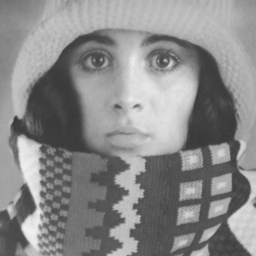
\includegraphics[width=0.5\linewidth]{../../images/grey/trui.png}
    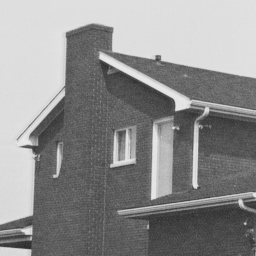
\includegraphics[width=0.5\linewidth]{../../images/grey/house.png}
    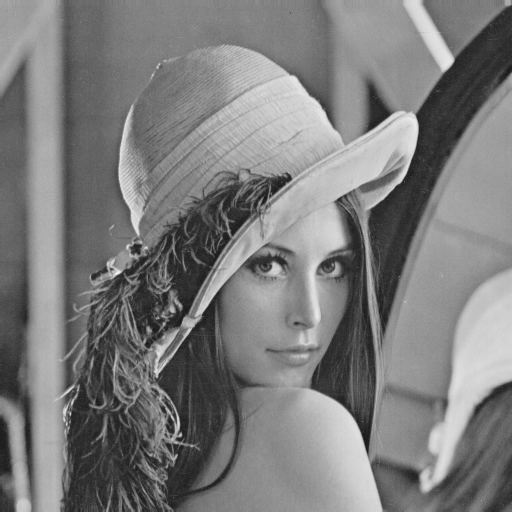
\includegraphics[width=0.5\linewidth]{../../images/grey/lena512.png}
    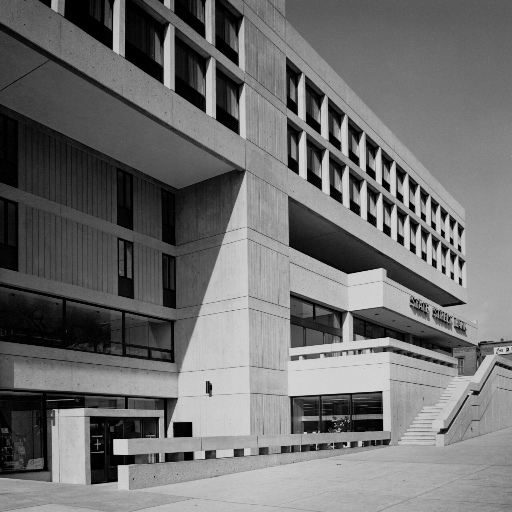
\includegraphics[width=0.5\linewidth]{../../images/grey/bank.png}
    \caption{Grey value images used for testing. From left to right and from top to bottom: \texttt{trui},
    \texttt{house}, \texttt{lena512}, \texttt{bank}}\label{fig:GreyValueImg}
\end{figure}
\begin{figure}[ht]
    
\includegraphics[width=0.32\linewidth]{../../images/binary/cat.png}
    
\includegraphics[width=0.32\linewidth]{../../images/binary/rect.png}
    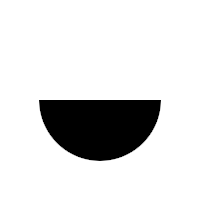
\includegraphics[width=0.32\linewidth]{../../images/binary/semicircle.png}
    
\includegraphics[width=0.32\linewidth]{../../images/binary/ellipse.png}
    
\includegraphics[width=0.32\linewidth]{../../images/binary/abstract1.png}
    
\includegraphics[width=0.32\linewidth]{../../images/binary/checkerboard32.png}
    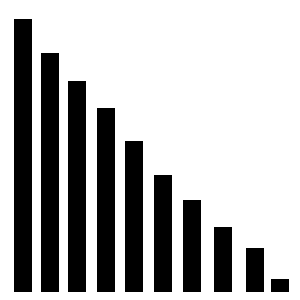
\includegraphics[width=0.32\linewidth]{../../images/binary/testlength.png}
    \caption{Binary images used for testing. From left to right and from top to bottom:
        \texttt{cat}, \texttt{rect},
    \texttt{semicircle}, \texttt{ellipse}, \texttt{abstract1}, \texttt{checkerboard32},
\texttt{testlength}}\label{fig:BinaryImg}
\end{figure}
\section{Parameter Selection}
As mentioned earlier, the optimal set of parameters is difficult to choose, that is why we have to
experiment a lot to find a decent approximation to this optimal set. In the following we will
therefore explain what the different parameters do, how that influences the image or mask quality
and ultimately, how we chose the parameters that we used to get our results.
First off, we talk about corner detection as this was the primary focus of our work. The parameter
choice was mainly fixed from the beginning as we used sets of parameters proven to be fairly
optimal in previous work by {<insert reference here>}. Nonetheless, we shortly go over the different
parameters and explain their influence.
\subsection{Corner Detection}
For corner detection there are not that many different parameters to play around with. In the
classical approach using the structure tensor (cf section \ref{sub:Corner}) we have only 3
parameters:
\begin{itemize}
    \item the noise scale $\sigma$
    \item the integration scale $\rho$ and
    \item a threshold parameter $T$ to filter out non-important corners
\end{itemize}
but as mentioned in section \ref{sec:Contribution}, we replaced the threshold by a percentile
parameter to make it more robust.
However, we introduced a new parameter $R$, that determines the size of the corner regions and
subsequently also the size of the region where the non-maximum suppression is performed in.

Regarding the noise scale, we generally want to choose it as large as necessary but keep it as small as
possible, meaning that we want to choose the smallest noise scale that gets rid of most of the
noise in the image since with a larger $\sigma$ 
one often faces the problem that the detected corners can not be located as accurately anymore,
since more and more relevant features are smoothed away (cf. scale space section). Another problem
is that the gaussian scale space (iterated gaussian smoothing) may even introduce new
corners.\cite{weickert96}
 Most of the time however, a $\sigma$ of 1 is sufficient enough to remove most of the noise and unnecessary
 details and still provide an accurate result.\\
Twe integration scale $\rho$ basically determines how `local' 
the corner detection is as it influences the size of the region structural information is averaged
in during the computation of the structure tensor. $\rho$ should always be chosen larger than the noise
scale $\sigma$, which leads us to a `standard' value of 2-2.5. In our experiments, these values
usually yielded the best results.\\
The newly introduced percentile parameter regulates the amount of corners that are ultimately being
detected since the percentile thresholding is applied \textit{after} the CNMS. 

\subsection{Inpainting}
The main parameters required by the inpainting process are 
\begin{itemize}
    \item the noise scale $\sigma$,
    \item the integration scale $\rho$,
    \item the contrast parameter $\lambda$, 
    \item the dissipativity parameter $\alpha$ and
    \item a non-negativity parameter $\gamma$.
\end{itemize}
The implementation of the algorithm that was provided by Joachim Weickert also requires some
technical parameters such as the choice of diffusivity function, time discretisation scheme, time
step size and iterative solver used for the semi-implicit time discretisation scheme.
 All these paramters were fixed beforehand. We used the Charbonnier diffusivity function mentioned
 in <theory>. As the other parameters are concerned, a semi-implicit scheme with a time step size
 of 1000 has been used. As an iterative solver for the system of equations that arises from the
 semi-implicit scheme a conjugate gradient solver with 200 iterations was used.
\\
If we recall from the theory section, when using EED, we do not need the integation scale, as the
integration scale only influences the radius of the structure tensor which is actually not needed
for this method of inpainting. Thus, this parameter will be fixed to 0.\\
The parameters $\alpha$ and $\gamma$ are purely numerical parameters that are used to 
stabilise the algorithm or rather help to ensure that the stencil weights of the discretisation of
the diffusion process meet certain requirements. A fairly optimal choice for these parameters has
been proposed in \cite{www13}, namely $\alpha=0.44, \gamma=0.98$.
In general, one could image the parameter $\alpha$ as a sharpness parameter: the larger the
$\alpha$ (but not larger than 0.5), the sharper the image. More on the nature of these two parameters can be read about in
\cite{www13, weickert96}.\\
Next up is the contrast parameter $\gamma$ that is required in the diffusivity function
\eqref{def:Diffusivity}. As already explained in the \ref{sec:Structure}, this parameter helps to
distinguish between edges and non-edges. For the EED inpainting this is especially important since
it basically determines how strongly edges will be continued into inpainting regions. We
experimented with different choices for this parameter but came to the conclusion that a fairly
small value yields the best results. In general, we used a value of 0.03 for most of the images,
but found that for a certain set of images, an even smaller value of 0.01 yielded better results.\\
Last but not least, the noise scale $\sigma$ determines how much the initial image is smoothed
before the computation of the image derivatives. In general, this parameter is always fixed at 1.0
as it only serves to regularise the differentiation process.
\section{Results}\label{sec:Results}

\chapter{Outlook}

\label{Outlook}


%----------------------------------------------------------------------------------------
%   THESIS CONTENT - APPENDICES
%----------------------------------------------------------------------------------------

\appendix % Cue to tell LaTeX that the following "chapters" are Appendices

% Include the appendices of the thesis as separate files from the Appendices folder
% Uncomment the lines as you write the Appendices

%\chapter{An Appendix}

Lorem ipsum dolor sit amet, consectetur adipiscing elit. Vivamus at pulvinar nisi. Phasellus hendrerit, diam placerat interdum iaculis, mauris justo cursus risus, in viverra purus eros at ligula. Ut metus justo, consequat a tristique posuere, laoreet nec nibh. Etiam et scelerisque mauris. Phasellus vel massa magna. Ut non neque id tortor pharetra bibendum vitae sit amet nisi. Duis nec quam quam, sed euismod justo. Pellentesque eu tellus vitae ante tempus malesuada. Nunc accumsan, quam in congue consequat, lectus lectus dapibus erat, id aliquet urna neque at massa. Nulla facilisi. Morbi ullamcorper eleifend posuere. Donec libero leo, faucibus nec bibendum at, mattis et urna. Proin consectetur, nunc ut imperdiet lobortis, magna neque tincidunt lectus, id iaculis nisi justo id nibh. Pellentesque vel sem in erat vulputate faucibus molestie ut lorem.

Quisque tristique urna in lorem laoreet at laoreet quam congue. Donec dolor turpis, blandit non imperdiet aliquet, blandit et felis. In lorem nisi, pretium sit amet vestibulum sed, tempus et sem. Proin non ante turpis. Nulla imperdiet fringilla convallis. Vivamus vel bibendum nisl. Pellentesque justo lectus, molestie vel luctus sed, lobortis in libero. Nulla facilisi. Aliquam erat volutpat. Suspendisse vitae nunc nunc. Sed aliquet est suscipit sapien rhoncus non adipiscing nibh consequat. Aliquam metus urna, faucibus eu vulputate non, luctus eu justo.

Donec urna leo, vulputate vitae porta eu, vehicula blandit libero. Phasellus eget massa et leo condimentum mollis. Nullam molestie, justo at pellentesque vulputate, sapien velit ornare diam, nec gravida lacus augue non diam. Integer mattis lacus id libero ultrices sit amet mollis neque molestie. Integer ut leo eget mi volutpat congue. Vivamus sodales, turpis id venenatis placerat, tellus purus adipiscing magna, eu aliquam nibh dolor id nibh. Pellentesque habitant morbi tristique senectus et netus et malesuada fames ac turpis egestas. Sed cursus convallis quam nec vehicula. Sed vulputate neque eget odio fringilla ac sodales urna feugiat.

Phasellus nisi quam, volutpat non ullamcorper eget, congue fringilla leo. Cras et erat et nibh placerat commodo id ornare est. Nulla facilisi. Aenean pulvinar scelerisque eros eget interdum. Nunc pulvinar magna ut felis varius in hendrerit dolor accumsan. Nunc pellentesque magna quis magna bibendum non laoreet erat tincidunt. Nulla facilisi.

Duis eget massa sem, gravida interdum ipsum. Nulla nunc nisl, hendrerit sit amet commodo vel, varius id tellus. Lorem ipsum dolor sit amet, consectetur adipiscing elit. Nunc ac dolor est. Suspendisse ultrices tincidunt metus eget accumsan. Nullam facilisis, justo vitae convallis sollicitudin, eros augue malesuada metus, nec sagittis diam nibh ut sapien. Duis blandit lectus vitae lorem aliquam nec euismod nisi volutpat. Vestibulum ornare dictum tortor, at faucibus justo tempor non. Nulla facilisi. Cras non massa nunc, eget euismod purus. Nunc metus ipsum, euismod a consectetur vel, hendrerit nec nunc.
%\include{Appendices/AppendixB}
%\include{Appendices/AppendixC}

%----------------------------------------------------------------------------------------
%   BIBLIOGRAPHY
%----------------------------------------------------------------------------------------

%\printbibliography[heading=bibintoc]

%----------------------------------------------------------------------------------------

\end{document}
